\documentclass[border=4pt]{standalone}
% shared style for all PyTBA topology diagrams (\input by each standalone file)
\usepackage{mathpazo}
\usepackage{amsmath}
\usepackage{tikz}
\usetikzlibrary{positioning,arrows.meta,calc,decorations.pathreplacing,fit,backgrounds}
\tikzset{
  host/.style={draw=blue!55!black, fill=blue!7, rounded corners=2pt, align=center,
               minimum height=9mm, minimum width=22mm, font=\small},
  blk/.style={draw=black!60, fill=black!4, rounded corners=2pt, align=center,
              minimum height=8mm, font=\small},
  chan/.style={draw=orange!70!black, fill=orange!8, rounded corners=2pt, align=center,
               minimum height=9mm, font=\small},
  lossbox/.style={draw=red!70!black, fill=red!6, rounded corners=2pt, align=center, font=\footnotesize},
  data/.style={-{Stealth[length=2.2mm]}, thick},
  ack/.style={-{Stealth[length=2mm]}, dashed, black!60},
  lbl/.style={font=\footnotesize, align=center},
  brace/.style={decorate, decoration={brace, amplitude=4pt}, thick, black!70},
}

\begin{document}
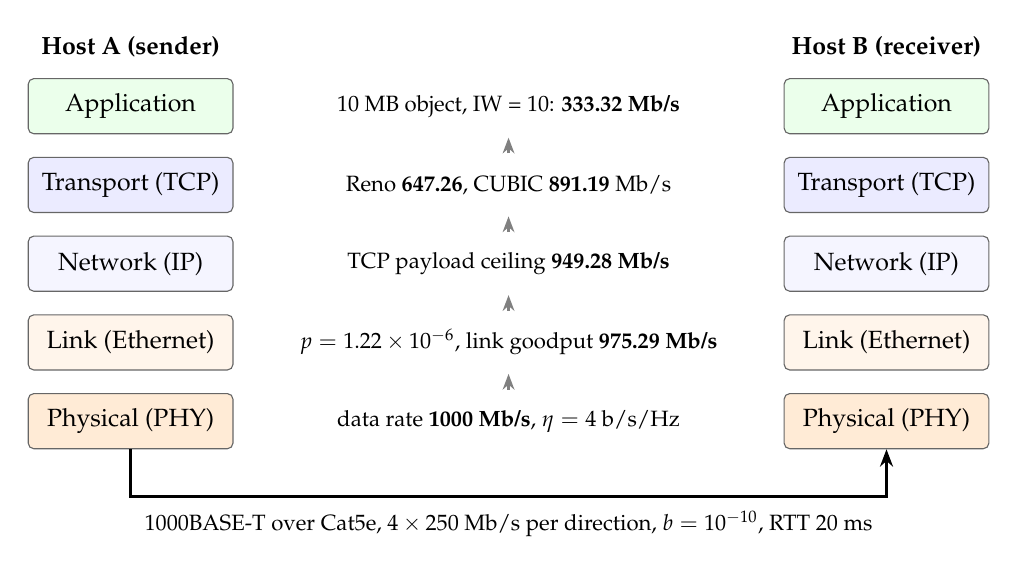
\begin{tikzpicture}[stk/.style={blk, minimum width=26mm, minimum height=7mm}]
\foreach \side/\x/\nm in {A/0/{Host A (sender)}, B/9.6/{Host B (receiver)}} {
  \node[stk, fill=green!8]  (app\side) at (\x,0)  {Application};
  \node[stk, fill=blue!8]   (tcp\side) at (\x,-1) {Transport (TCP)};
  \node[stk, fill=blue!4]   (ip\side)  at (\x,-2) {Network (IP)};
  \node[stk, fill=orange!8] (lnk\side) at (\x,-3) {Link (Ethernet)};
  \node[stk, fill=orange!16](phy\side) at (\x,-4) {Physical (PHY)};
  \node[font=\small\bfseries] at (\x,0.75) {\nm};
}
\draw[data, line width=1.2pt] (phyA.south) -- ++(0,-0.6) -| (phyB.south);
\node[lbl] at (4.8,-5.3) {1000BASE-T over Cat5e, $4\times250$ Mb/s per direction, $b=10^{-10}$, RTT 20 ms};
\foreach \y/\txt in {0/{10 MB object, IW = 10: \textbf{333.32 Mb/s}},
                     -1/{Reno \textbf{647.26}, CUBIC \textbf{891.19} Mb/s},
                     -2/{TCP payload ceiling \textbf{949.28 Mb/s}},
                     -3/{$p=1.22\times10^{-6}$, link goodput \textbf{975.29 Mb/s}},
                     -4/{data rate \textbf{1000 Mb/s}, $\eta=4$ b/s/Hz}}
  \node[lbl] at (4.8,\y) {\txt};
\draw[-{Stealth[length=2mm]}, black!50, thick] (4.8,-3.6) -- (4.8,-3.4);
\draw[-{Stealth[length=2mm]}, black!50, thick] (4.8,-2.6) -- (4.8,-2.4);
\draw[-{Stealth[length=2mm]}, black!50, thick] (4.8,-1.6) -- (4.8,-1.4);
\draw[-{Stealth[length=2mm]}, black!50, thick] (4.8,-0.6) -- (4.8,-0.4);
\end{tikzpicture}
\end{document}
